\section{Deus Ex: Human Revolution}

\begin{figure}[htbp]
\begin{center}
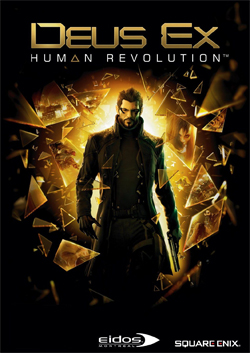
\includegraphics[width=.60\textwidth]{./imagenes/deusex.jpg}
\caption{Deus Ex: Human Revolution}
\label{Deus Ex: Human Revolution}
\end{center}
\end{figure}
Deus Ex: Human Revolution\footnote{\url{http://www.deusex.com/}}  es la prequela del aclamado "Deus Ex", lanzada en Agosto del 2011 por Eidos Montreal. Es un juego que se lleva a cabo en un futuro no muy distante, donde las aumentaciones (implantes físicos) son cosas del día a día, y que dan poder a quién las tenga.
En medio de todo esto se encuentra el protagonista, Adam Jensen, el cual se ve inmerso en un complot que abarca el destino de la humanidad.

\subsubsection{¿Por qué es uno de mis juegos favoritos?}
\begin{itemize}
\item[Luis Vasquez] Con un fanático de la serie, me fué natural comprar este juego en el día de lanzamiento, y no fui decepcionado. A parte de la gran trama que este juego ofrece , la cual no le pide favores a la del original, este logra modernizar todos los aspectos de jugabilidad
de  Deus Ex, asi como ofrecer al jugador varias opciones de juego, uno puede elegir entre sigilosamente inflitrarse en la base enemiga sin ser visto, o simplemente asesinar a sangre fría a cualquiera que se te cruze en tu camino.
\end{itemize}
